\documentclass{standalone}
\usepackage{tikz}
\usetikzlibrary{patterns, positioning}
\usepackage[sfdefault]{ClearSans} %% option 'sfdefault' activates Clear Sans as the default text font
\usepackage[T1]{fontenc}

\begin{document}
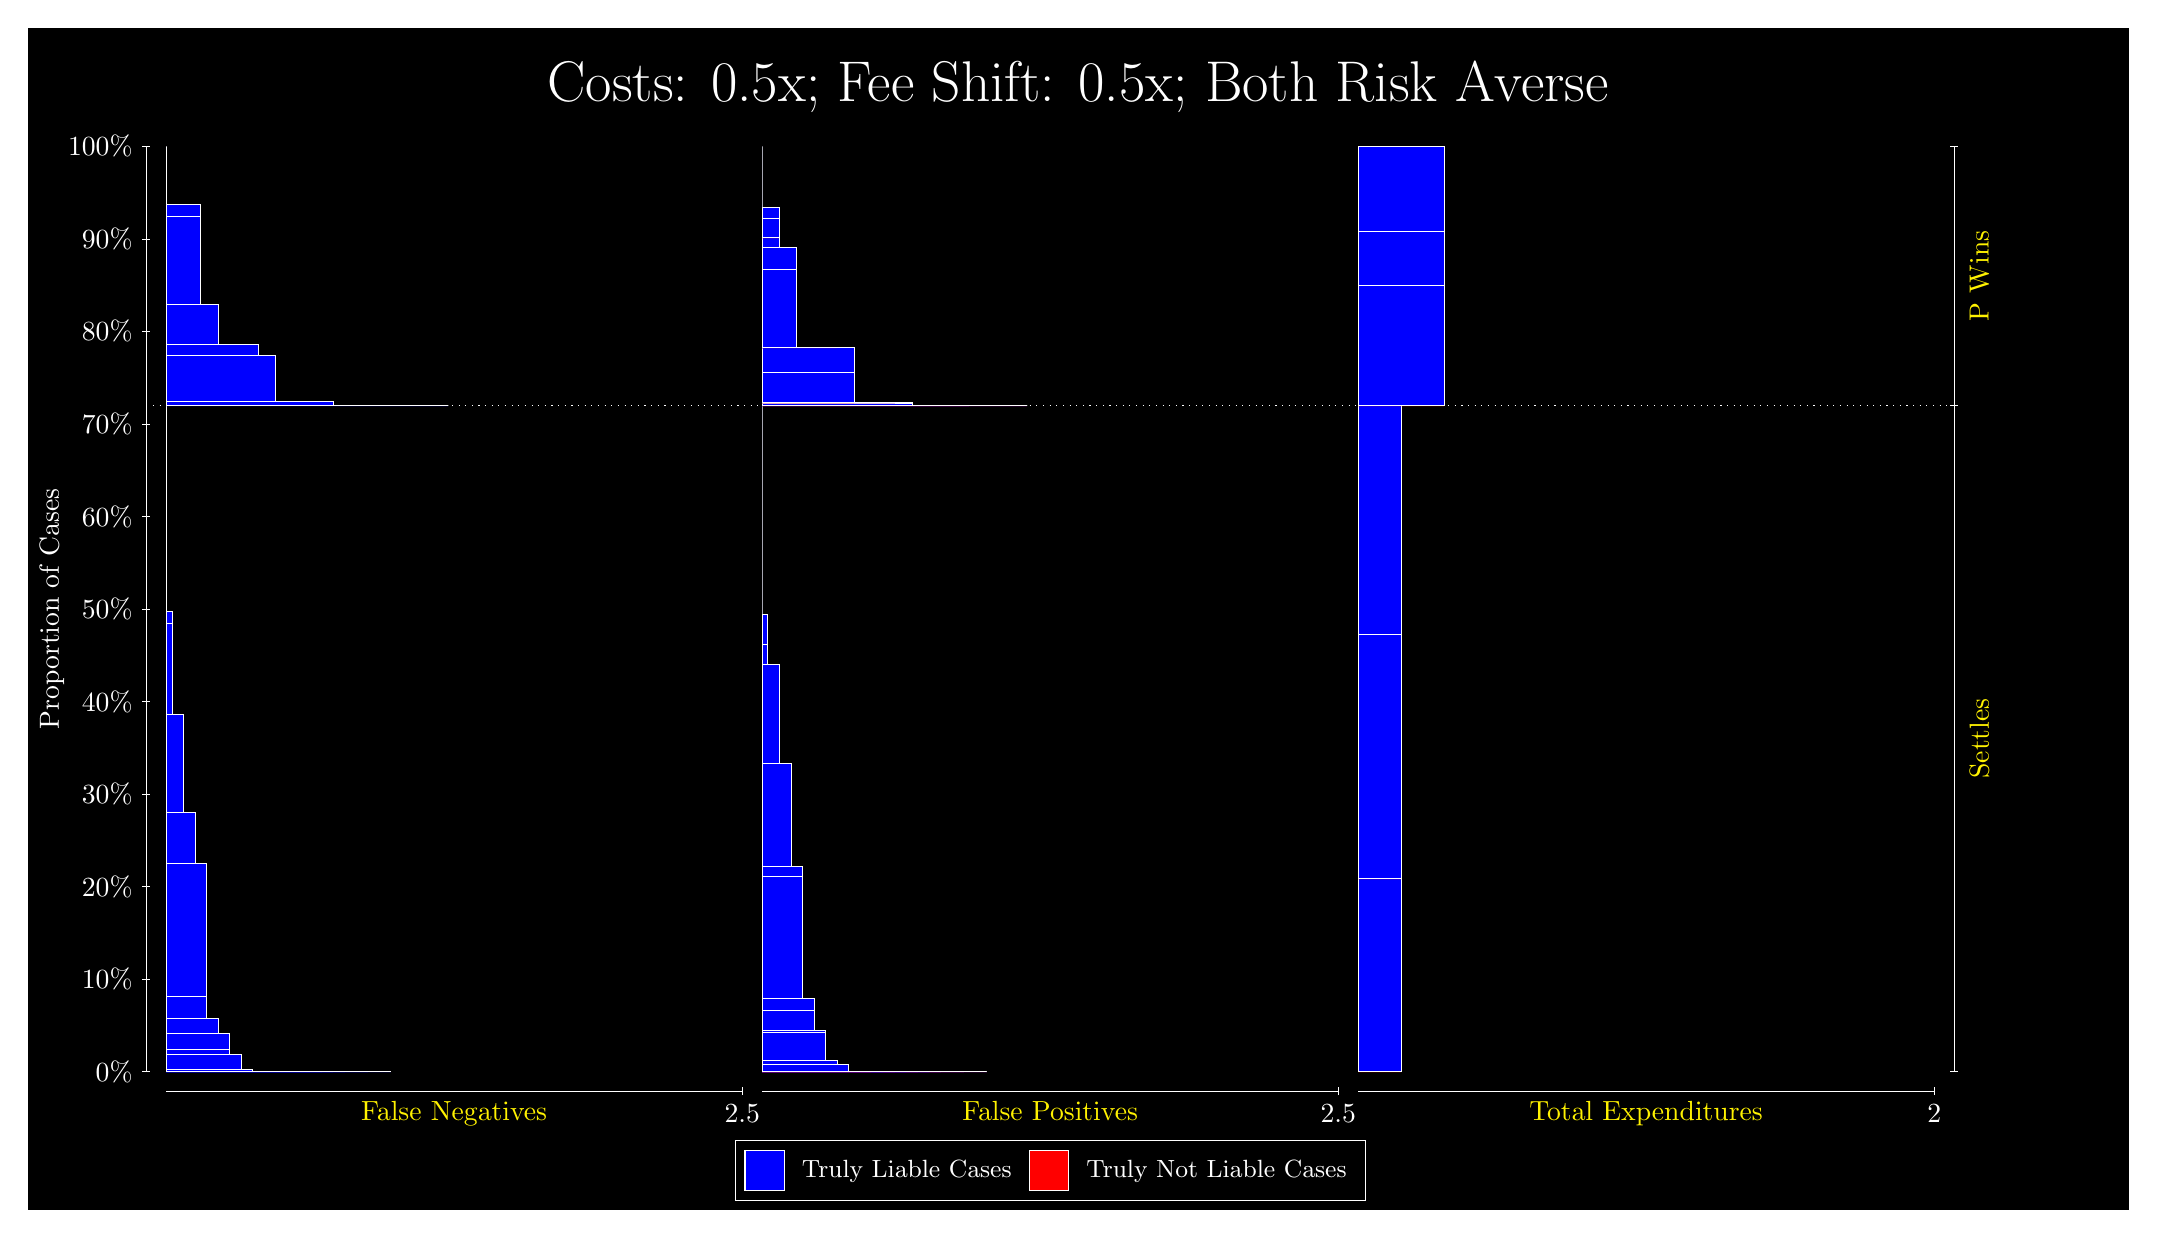
\begin{tikzpicture}
\draw[fill=black] (0,0) rectangle (26.667,15);
\draw[text=white] (0,13.5) rectangle (26.667,15) node[midway] {\huge Costs: 0.5x; Fee Shift: 0.5x; Both Risk Averse};
\draw[white, very thin] (1.5,1.75) -- (1.5,13.5);
\node[rotate=90, text=white, anchor=center] at (0.3, 7.625) {Proportion of Cases};
\draw[white, very thin] (1.45,1.75) -- (1.55,1.75);
\node[text=white, anchor=east] at (1.45, 1.75) {0\%};
\draw[white, very thin] (1.45,2.925) -- (1.55,2.925);
\node[text=white, anchor=east] at (1.45, 2.925) {10\%};
\draw[white, very thin] (1.45,4.1) -- (1.55,4.1);
\node[text=white, anchor=east] at (1.45, 4.1) {20\%};
\draw[white, very thin] (1.45,5.275) -- (1.55,5.275);
\node[text=white, anchor=east] at (1.45, 5.275) {30\%};
\draw[white, very thin] (1.45,6.45) -- (1.55,6.45);
\node[text=white, anchor=east] at (1.45, 6.45) {40\%};
\draw[white, very thin] (1.45,7.625) -- (1.55,7.625);
\node[text=white, anchor=east] at (1.45, 7.625) {50\%};
\draw[white, very thin] (1.45,8.8) -- (1.55,8.8);
\node[text=white, anchor=east] at (1.45, 8.8) {60\%};
\draw[white, very thin] (1.45,9.975) -- (1.55,9.975);
\node[text=white, anchor=east] at (1.45, 9.975) {70\%};
\draw[white, very thin] (1.45,11.15) -- (1.55,11.15);
\node[text=white, anchor=east] at (1.45, 11.15) {80\%};
\draw[white, very thin] (1.45,12.325) -- (1.55,12.325);
\node[text=white, anchor=east] at (1.45, 12.325) {90\%};
\draw[white, very thin] (1.45,13.5) -- (1.55,13.5);
\node[text=white, anchor=east] at (1.45, 13.5) {100\%};

\draw[white, very thin] (24.457,1.75) -- (24.457,13.5);
\draw[white, very thin] (24.407,1.75) -- (24.507,1.75);
\node[anchor=west] at (24.407, 1.75) {};
\draw[white, very thin] (24.407,10.208) -- (24.507,10.208);
\node[anchor=west] at (24.407, 10.208) {};
\draw[white, very thin] (24.407,13.5) -- (24.507,13.5);
\node[anchor=west] at (24.407, 13.5) {};

\draw[white, very thin, fill=blue] (1.75,1.75) rectangle (4.6044,1.75);
\draw[white, very thin, fill=blue] (1.75,1.75) rectangle (4.3116,1.75);
\draw[white, very thin, fill=blue] (1.75,1.75) rectangle (4.0188,1.75);
\draw[white, very thin, fill=blue] (1.75,1.75) rectangle (3.8725,1.75);
\draw[white, very thin, fill=blue] (1.75,1.75) rectangle (3.7261,1.75);
\draw[white, very thin, fill=blue] (1.75,1.75) rectangle (3.5797,1.75);
\draw[white, very thin, fill=blue] (1.75,1.75) rectangle (3.4333,1.7504);
\draw[white, very thin, fill=blue] (1.75,1.7504) rectangle (3.287,1.7504);
\draw[white, very thin, fill=blue] (1.75,1.7504) rectangle (3.1406,1.7507);
\draw[white, very thin, fill=blue] (1.75,1.7507) rectangle (2.9942,1.7507);
\draw[white, very thin, fill=blue] (1.75,1.7507) rectangle (2.9942,1.7523);
\draw[white, very thin, fill=blue] (1.75,1.7523) rectangle (2.8478,1.7805);
\draw[white, very thin, fill=blue] (1.75,1.7805) rectangle (2.7015,1.9664);
\draw[white, very thin, fill=blue] (1.75,1.9664) rectangle (2.5551,2.027);
\draw[white, very thin, fill=blue] (1.75,2.027) rectangle (2.5551,2.2409);
\draw[white, very thin, fill=blue] (1.75,2.2409) rectangle (2.4087,2.4262);
\draw[white, very thin, fill=blue] (1.75,2.4262) rectangle (2.2623,2.4265);
\draw[white, very thin, fill=blue] (1.75,2.4265) rectangle (2.2623,2.7079);
\draw[white, very thin, fill=blue] (1.75,2.7079) rectangle (2.2623,4.3978);
\draw[white, very thin, fill=blue] (1.75,4.3978) rectangle (2.1159,5.0386);
\draw[white, very thin, fill=blue] (1.75,5.0386) rectangle (1.9696,6.2892);
\draw[white, very thin, fill=blue] (1.75,6.2892) rectangle (1.8232,7.446);
\draw[white, very thin, fill=blue] (1.75,7.446) rectangle (1.8232,7.5978);
\draw[white, very thin, fill=red] (1.75,7.5978) rectangle (1.75,7.5978);
\draw[white, very thin, fill=blue] (1.75,7.5978) rectangle (1.75,10.208);
\draw[white, very thin, fill=blue] (1.75,10.208) rectangle (5.3362,10.208);
\draw[white, very thin, fill=blue] (1.75,10.208) rectangle (4.6044,10.209);
\draw[white, very thin, fill=blue] (1.75,10.209) rectangle (4.3848,10.209);
\draw[white, very thin, fill=blue] (1.75,10.209) rectangle (3.8725,10.266);
\draw[white, very thin, fill=blue] (1.75,10.266) rectangle (3.6529,10.266);
\draw[white, very thin, fill=blue] (1.75,10.266) rectangle (3.1406,10.852);
\draw[white, very thin, fill=blue] (1.75,10.852) rectangle (2.921,10.982);
\draw[white, very thin, fill=blue] (1.75,10.982) rectangle (2.4087,11.496);
\draw[white, very thin, fill=blue] (1.75,11.496) rectangle (2.1891,12.606);
\draw[white, very thin, fill=blue] (1.75,12.606) rectangle (2.1891,12.764);
\draw[white, very thin, fill=red] (1.75,12.764) rectangle (1.75,12.764);
\draw[white, very thin, fill=blue] (1.75,12.764) rectangle (1.75,13.5);
\draw[white, very thin, fill=red] (9.3189,1.75) rectangle (12.173,1.75);
\draw[white, very thin, fill=blue] (9.3189,1.75) rectangle (12.173,1.75);
\draw[white, very thin, fill=red] (9.3189,1.75) rectangle (11.88,1.75);
\draw[white, very thin, fill=blue] (9.3189,1.75) rectangle (11.88,1.75);
\draw[white, very thin, fill=red] (9.3189,1.75) rectangle (11.588,1.75);
\draw[white, very thin, fill=blue] (9.3189,1.75) rectangle (11.588,1.75);
\draw[white, very thin, fill=blue] (9.3189,1.75) rectangle (11.441,1.75);
\draw[white, very thin, fill=red] (9.3189,1.75) rectangle (11.295,1.75);
\draw[white, very thin, fill=blue] (9.3189,1.75) rectangle (11.295,1.75);
\draw[white, very thin, fill=blue] (9.3189,1.75) rectangle (11.149,1.75);
\draw[white, very thin, fill=red] (9.3189,1.75) rectangle (11.002,1.75);
\draw[white, very thin, fill=blue] (9.3189,1.75) rectangle (11.002,1.75);
\draw[white, very thin, fill=blue] (9.3189,1.75) rectangle (10.856,1.75);
\draw[white, very thin, fill=red] (9.3189,1.75) rectangle (10.709,1.75);
\draw[white, very thin, fill=blue] (9.3189,1.75) rectangle (10.709,1.7507);
\draw[white, very thin, fill=red] (9.3189,1.7507) rectangle (10.709,1.7507);
\draw[white, very thin, fill=blue] (9.3189,1.7507) rectangle (10.709,1.7509);
\draw[white, very thin, fill=blue] (9.3189,1.7509) rectangle (10.563,1.7512);
\draw[white, very thin, fill=red] (9.3189,1.7512) rectangle (10.417,1.7512);
\draw[white, very thin, fill=blue] (9.3189,1.7512) rectangle (10.417,1.8367);
\draw[white, very thin, fill=blue] (9.3189,1.8367) rectangle (10.27,1.8963);
\draw[white, very thin, fill=red] (9.3189,1.8963) rectangle (10.124,1.8963);
\draw[white, very thin, fill=blue] (9.3189,1.8963) rectangle (10.124,2.2528);
\draw[white, very thin, fill=blue] (9.3189,2.2528) rectangle (10.124,2.2725);
\draw[white, very thin, fill=blue] (9.3189,2.2725) rectangle (9.9776,2.5266);
\draw[white, very thin, fill=blue] (9.3189,2.5266) rectangle (9.9776,2.6864);
\draw[white, very thin, fill=red] (9.3189,2.6864) rectangle (9.8312,2.6864);
\draw[white, very thin, fill=blue] (9.3189,2.6864) rectangle (9.8312,4.2336);
\draw[white, very thin, fill=blue] (9.3189,4.2336) rectangle (9.8312,4.3603);
\draw[white, very thin, fill=blue] (9.3189,4.3603) rectangle (9.6848,5.6689);
\draw[white, very thin, fill=blue] (9.3189,5.6689) rectangle (9.5384,6.9195);
\draw[white, very thin, fill=blue] (9.3189,6.9195) rectangle (9.3921,7.1725);
\draw[white, very thin, fill=blue] (9.3189,7.1725) rectangle (9.3921,7.5603);
\draw[white, very thin, fill=blue] (9.3189,7.5603) rectangle (9.3189,10.208);
\draw[white, very thin, fill=red] (9.3189,10.208) rectangle (12.686,10.208);
\draw[white, very thin, fill=blue] (9.3189,10.208) rectangle (12.686,10.208);
\draw[white, very thin, fill=red] (9.3189,10.208) rectangle (11.954,10.208);
\draw[white, very thin, fill=blue] (9.3189,10.208) rectangle (11.954,10.208);
\draw[white, very thin, fill=blue] (9.3189,10.208) rectangle (11.954,10.209);
\draw[white, very thin, fill=red] (9.3189,10.209) rectangle (11.222,10.209);
\draw[white, very thin, fill=blue] (9.3189,10.209) rectangle (11.222,10.232);
\draw[white, very thin, fill=blue] (9.3189,10.232) rectangle (11.222,10.246);
\draw[white, very thin, fill=red] (9.3189,10.246) rectangle (11.002,10.246);
\draw[white, very thin, fill=blue] (9.3189,10.246) rectangle (11.002,10.246);
\draw[white, very thin, fill=red] (9.3189,10.246) rectangle (10.49,10.246);
\draw[white, very thin, fill=blue] (9.3189,10.246) rectangle (10.49,10.63);
\draw[white, very thin, fill=blue] (9.3189,10.63) rectangle (10.49,10.944);
\draw[white, very thin, fill=red] (9.3189,10.944) rectangle (10.27,10.944);
\draw[white, very thin, fill=blue] (9.3189,10.944) rectangle (10.27,10.944);
\draw[white, very thin, fill=blue] (9.3189,10.944) rectangle (10.27,10.944);
\draw[white, very thin, fill=blue] (9.3189,10.944) rectangle (9.758,11.935);
\draw[white, very thin, fill=blue] (9.3189,11.935) rectangle (9.758,12.212);
\draw[white, very thin, fill=blue] (9.3189,12.212) rectangle (9.5384,12.341);
\draw[white, very thin, fill=red] (9.3189,12.341) rectangle (9.5384,12.341);
\draw[white, very thin, fill=blue] (9.3189,12.341) rectangle (9.5384,12.58);
\draw[white, very thin, fill=blue] (9.3189,12.58) rectangle (9.5384,12.726);
\draw[white, very thin, fill=blue] (9.3189,12.726) rectangle (9.3189,13.5);
\draw[white, very thin, fill=red] (16.888,1.75) rectangle (17.437,1.75);
\draw[white, very thin, fill=blue] (16.888,1.75) rectangle (17.437,4.201);
\draw[white, very thin, fill=red] (16.888,4.201) rectangle (17.437,4.201);
\draw[white, very thin, fill=blue] (16.888,4.201) rectangle (17.437,7.3031);
\draw[white, very thin, fill=red] (16.888,7.3031) rectangle (17.437,7.3031);
\draw[white, very thin, fill=blue] (16.888,7.3031) rectangle (17.437,10.208);
\draw[white, very thin, fill=red] (16.888,10.208) rectangle (17.986,10.208);
\draw[white, very thin, fill=blue] (16.888,10.208) rectangle (17.986,11.737);
\draw[white, very thin, fill=red] (16.888,11.737) rectangle (17.986,11.737);
\draw[white, very thin, fill=blue] (16.888,11.737) rectangle (17.986,12.423);
\draw[white, very thin, fill=red] (16.888,12.423) rectangle (17.986,12.423);
\draw[white, very thin, fill=blue] (16.888,12.423) rectangle (17.986,13.5);
\draw[white, dotted] (1.5,10.208) -- (24.457,10.208);
\draw[white, very thin] (1.75,1.5) -- (9.0689,1.5);
\node[text=yellow, anchor=north] at (5.4094, 1.5) {False Negatives};
\draw[white, very thin] (9.0689,1.45) -- (9.0689,1.55);
\node[text=white, anchor=north] at (9.0689, 1.45) {2.5};

\draw[white, very thin] (9.3189,1.5) -- (16.638,1.5);
\node[text=yellow, anchor=north] at (12.978, 1.5) {False Positives};
\draw[white, very thin] (16.638,1.45) -- (16.638,1.55);
\node[text=white, anchor=north] at (16.638, 1.45) {2.5};

\draw[white, very thin] (16.888,1.5) -- (24.207,1.5);
\node[text=yellow, anchor=north] at (20.547, 1.5) {Total Expenditures};
\draw[white, very thin] (24.207,1.45) -- (24.207,1.55);
\node[text=white, anchor=north] at (24.207, 1.45) {2};

\node[text=yellow, centered, rotate=90] at (24.777, 5.9791) {Settles};
\node[text=yellow, centered, rotate=90] at (24.777, 11.854) {P Wins};

\draw (12.978300999999998,1.5) node[draw=none] (baseCoordinate) {};
\begin{scope}[align=center]
        \matrix[scale=0.5, draw=white, below=0.5cm of baseCoordinate, nodes={draw}, column sep=0.1cm]{
            \node[rectangle, draw, minimum width=0.5cm, minimum height=0.5cm, fill=blue] {}; &
            \node[draw=none, font=\small, text=white] (B) {Truly Liable Cases}; &
            \node[rectangle, draw, minimum width=0.5cm, minimum height=0.5cm, fill=red] {}; &
            \node[draw=none, font=\small, text=white] (B) {Truly Not Liable Cases}; \\
            };
\end{scope}

\end{tikzpicture}
\end{document}